\section{Decomposition of Graphs}

\subsection{DFS in Undirected Graphs}

\begin{definition}[explore]
Finding all nodes reachable from a particular node.
	\begin{lstlisting}[mathescape=true, language=Octave]
procedure explore(G, v):
	% Input: Graph G = (V, E), v a node in V
	% Output: u.visited is set true for all node u reachable from v
	v.visited = true
	previsit(v)
	foreach (v, u) in E:
		if not u.visited: explore(G, u)
	postvisit(v)
\end{lstlisting}
Where previsit(v) and postvisit(v) denotes the "time" $\tau$ before and after v is explored, respectively.
\end{definition}

\begin{definition}[DFS]
Based on Definition of explore, a DFS procedure is as follows:
\begin{lstlisting}[mathescape=true, language=Octave]
procedure DFS(G)
	% Input: Graph G = (V, E)
	forall v in V:
		if not v.visited: explore(v)
\end{lstlisting}
\end{definition}

\begin{definition}[ordering]
The previsit and postvisit ordering is defined as follows:
\begin{lstlisting}[mathescape=true, language=Octave]
procedure previsit(v)
	pre[v] = clock
	clock += 1
procedure postvisit(v)
	post[v] = clock
	clock += 1
\end{lstlisting}
\end{definition}

\begin{remark}
The implementation of a DFS uses a stack and DFS's runtime is $O(|V|+|E|)$.
\end{remark}

\subsection{DFS in Directed Graphs}

\begin{definition}[Type of Edges]
There four types of edges:
\begin{itemize}
	\item Tree edges are part of the DFS forest
	\item Forward edges lead to a nonchild descendant
	\item Back edges lead to a not-direct ancestor
	\item Cross edges lead to a node that is neither descendant nor ancestor, a node that has already been completely explored.
\end{itemize}
An edge (u, v) in E is:
\begin{itemize}
	\item Forward if pre(u) $<$ pre(v) $<$ post(v) $<$ post(u)
	\item Back if pre(v) $<$ pre(u) $<$ post(u) $<$ post(v)
	\item Cross if pre(v) $<$ post(v) $<$ pre(u) $<$ post(u)
\end{itemize}
\end{definition}

\begin{definition}
	A directed graph has a cycle iff its DFS reveals a back edge. If the DFS of a directed graph reveals no back edge, the graph is a Directed Acyclic Graph (DAG).
\end{definition}

\begin{theorem}
	All DAG can be linearized (topologically sorted). That is, if G(V, E) is a DAG with (u, v) in E, then post(u) $>$ post(v).
\end{theorem}

\begin{theorem}
	All DAG must have at least one source (a node with no ingoing edges) and at least one sink (a node with no outgoing edges). 
\end{theorem}

\begin{theorem}
	A DAG, after delete one of its sources, is still a DAG.
\end{theorem}

\begin{theorem}
	A DAG have one or more possible linearizations. The following algorithm,
\begin{lstlisting}[mathescape=true, language=Octave]
procedure linearize(G)
	while G:
		find a source s in G
		pop s
\end{lstlisting}
Is guaranteed to give a linearization.
\end{theorem}

\begin{remark}
	In a DF traverse of a binary tree, the visiting order of nodes can be found by labeling the graph like follows: \\
	\begin{center}
		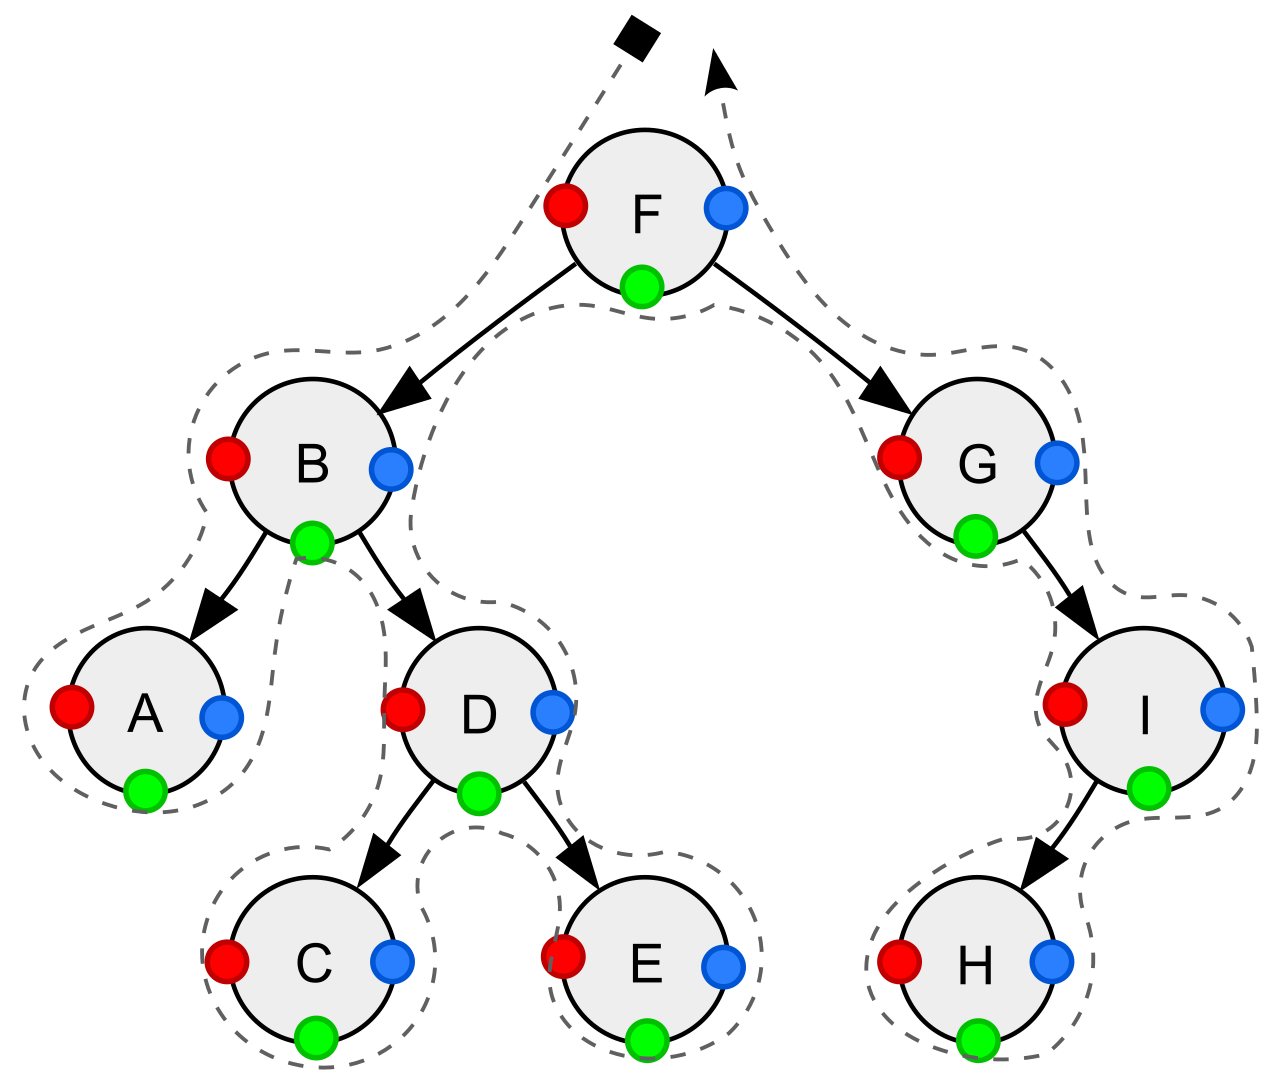
\includegraphics[scale=0.2]{images/dfs_order.png} \\
	\end{center}
	Where red dots denote preorder, green dots denote in-order, and blue dots denote post-order.
\end{remark}

\subsection{Strongly Connected Components}